\documentclass[a4paper,12pt]{article}
\usepackage{../../synopsis/my_preamble}

\geometry{
    includehead,
    headsep=\baselineskip,
}

\usepackage{pgfplots}

\DeclareUnicodeCharacter{2212}{-}
\usepgfplotslibrary{groupplots,dateplot}
\usetikzlibrary{patterns,shapes.arrows}
\pgfplotsset{compat=newest}

\pagestyle{fancy}
\fancyhf{}
\setlength{\headheight}{30pt}
\lhead{$\bm{\mathcal{H}}$\textbf{omework~\#5}\\\textbf{Graph~Theory}}
\rhead{\textbf{sltKaguya,~Group}\\\textbf{April~30~---~\today}}

\newcommand{\graph}[1][G]{\mathcal{#1}}

\newcommand{\op}[1]{\operatorname*{#1}}

\newcommand{\minDegree}[1]{\delta(#1)}
\newcommand{\maxDegree}[1]{\Delta(#1)}
\newcommand{\graphRadius}[1]{\op{rad}(#1)}
\newcommand{\graphDiameter}[1]{\op{diam}(#1)}
\newcommand{\graphGirth}[1]{\op{girth}(#1)}
\newcommand{\graphCenter}[1]{\op{center}(#1)}
\newcommand{\graphCentroid}[1]{\op{centroid}(#1)}
\newcommand{\vertexConnectivity}[1]{\varkappa(#1)}
\newcommand{\edgeConnectivity}[1]{\lambda(#1)}

\newcommand{\dist}[1]{\op{dist}(#1)}
\newcommand{\blockGraph}[1]{\op{B}(#1)}
\newcommand{\eccentricity}[1]{\varepsilon(#1)}

\begin{document}

\begin{tasks}
    \item The graph\footnote{Hereinafter, \enquote{graphs} are \enquote{simple, finite, undirected and unweighted}, unless stated otherwise.} of Europe $\graph^{*} = \langle V, E\rangle$ is defined as follows: each vertex $v \in V$ is a Europe country\footnote{\url{https://simple.wikipedia.org/wiki/List_of_European_countries} used as reference.}; two vertices are adjacent $(\{u, v\} \in E)$ if the corresponding countries share a land border. Let $\graph$ be the largest connected component of $\graph^{*}$.
    
    \begin{subtasks}
        \item Draw $\graph^{*}$ with the minimum number of intersecting edges.
        
            \begingroup
            \tikzset{every picture/.style={scale=1.5}}%
            % This file was created with tikzplotlib v0.10.1.
\begin{tikzpicture}

\definecolor{darkgray176}{RGB}{176,176,176}

\begin{axis}[
scaled x ticks=manual:{}{\pgfmathparse{#1}},
scaled y ticks=manual:{}{\pgfmathparse{#1}},
tick align=outside,
x grid style={darkgray176},
xmajorticks=false,
xmin=-1360.95, xmax=4192.95,
xtick style={color=black},
xticklabels={},
y grid style={darkgray176},
ymajorticks=false,
ymin=-1268.67, ymax=1700.67,
ytick style={color=black},
yticklabels={}
]
\path [draw=black]
(axis cs:1651,-693)
--(axis cs:2054,-1011);

\path [draw=black]
(axis cs:1651,-693)
--(axis cs:1741,-525);

\path [draw=black]
(axis cs:1651,-693)
--(axis cs:1775,-596);

\path [draw=black]
(axis cs:1651,-693)
--(axis cs:1588,-574);

\path [draw=black]
(axis cs:107,-575)
--(axis cs:251,127);

\path [draw=black]
(axis cs:107,-575)
--(axis cs:-367,-741);

\path [draw=black]
(axis cs:3711,-166)
--(axis cs:3656,-1);

\path [draw=black]
(axis cs:3711,-166)
--(axis cs:2786,-589);

\path [draw=black]
(axis cs:1289,43)
--(axis cs:1135,242);

\path [draw=black]
(axis cs:1289,43)
--(axis cs:1045,508);

\path [draw=black]
(axis cs:1289,43)
--(axis cs:1501,-11);

\path [draw=black]
(axis cs:1289,43)
--(axis cs:1025,-681);

\path [draw=black]
(axis cs:1289,43)
--(axis cs:778,-96);

\path [draw=black]
(axis cs:1289,43)
--(axis cs:1345,43);

\path [draw=black]
(axis cs:1289,43)
--(axis cs:1167,-206);

\path [draw=black]
(axis cs:1289,43)
--(axis cs:620,-117);

\path [draw=black]
(axis cs:1958,798)
--(axis cs:1669,1081);

\path [draw=black]
(axis cs:1958,798)
--(axis cs:1795,850);

\path [draw=black]
(axis cs:1958,798)
--(axis cs:1563,531);

\path [draw=black]
(axis cs:1958,798)
--(axis cs:2506,1194);

\path [draw=black]
(axis cs:1958,798)
--(axis cs:2254,480);

\path [draw=black]
(axis cs:415,331)
--(axis cs:251,127);

\path [draw=black]
(axis cs:415,331)
--(axis cs:1045,508);

\path [draw=black]
(axis cs:415,331)
--(axis cs:533,186);

\path [draw=black]
(axis cs:415,331)
--(axis cs:468,497);

\path [draw=black]
(axis cs:1499,-422)
--(axis cs:1284,-226);

\path [draw=black]
(axis cs:1499,-422)
--(axis cs:1588,-574);

\path [draw=black]
(axis cs:1499,-422)
--(axis cs:1651,-292);

\path [draw=black]
(axis cs:1918,-493)
--(axis cs:2054,-1011);

\path [draw=black]
(axis cs:1918,-493)
--(axis cs:1775,-596);

\path [draw=black]
(axis cs:1918,-493)
--(axis cs:2101,-253);

\path [draw=black]
(axis cs:1918,-493)
--(axis cs:1651,-292);

\path [draw=black]
(axis cs:1918,-493)
--(axis cs:2786,-589);

\path [draw=black]
(axis cs:1284,-226)
--(axis cs:1501,-11);

\path [draw=black]
(axis cs:1284,-226)
--(axis cs:1588,-574);

\path [draw=black]
(axis cs:1284,-226)
--(axis cs:1651,-292);

\path [draw=black]
(axis cs:1284,-226)
--(axis cs:1167,-206);

\path [draw=black]
(axis cs:1135,242)
--(axis cs:1045,508);

\path [draw=black]
(axis cs:1135,242)
--(axis cs:1563,531);

\path [draw=black]
(axis cs:1135,242)
--(axis cs:1345,43);

\path [draw=black]
(axis cs:977,856)
--(axis cs:1045,508);

\path [draw=black]
(axis cs:1648,1361)
--(axis cs:1669,1081);

\path [draw=black]
(axis cs:1648,1361)
--(axis cs:2506,1194);

\path [draw=black]
(axis cs:1643,1443)
--(axis cs:857,1329);

\path [draw=black]
(axis cs:1643,1443)
--(axis cs:1274,1289);

\path [draw=black]
(axis cs:1643,1443)
--(axis cs:2506,1194);

\path [draw=black]
(axis cs:251,127)
--(axis cs:1045,508);

\path [draw=black]
(axis cs:251,127)
--(axis cs:1025,-681);

\path [draw=black]
(axis cs:251,127)
--(axis cs:533,186);

\path [draw=black]
(axis cs:251,127)
--(axis cs:604,-474);

\path [draw=black]
(axis cs:251,127)
--(axis cs:-367,-741);

\path [draw=black]
(axis cs:251,127)
--(axis cs:620,-117);

\path [draw=black]
(axis cs:3656,-1)
--(axis cs:2506,1194);

\path [draw=black]
(axis cs:3656,-1)
--(axis cs:2786,-589);

\path [draw=black]
(axis cs:1045,508)
--(axis cs:533,186);

\path [draw=black]
(axis cs:1045,508)
--(axis cs:468,497);

\path [draw=black]
(axis cs:1045,508)
--(axis cs:1563,531);

\path [draw=black]
(axis cs:1045,508)
--(axis cs:620,-117);

\path [draw=black]
(axis cs:2054,-1011)
--(axis cs:2786,-589);

\path [draw=black]
(axis cs:2054,-1011)
--(axis cs:1775,-596);

\path [draw=black]
(axis cs:1501,-11)
--(axis cs:2101,-253);

\path [draw=black]
(axis cs:1501,-11)
--(axis cs:1651,-292);

\path [draw=black]
(axis cs:1501,-11)
--(axis cs:1345,43);

\path [draw=black]
(axis cs:1501,-11)
--(axis cs:1167,-206);

\path [draw=black]
(axis cs:1501,-11)
--(axis cs:2254,480);

\path [draw=black]
(axis cs:-257,715)
--(axis cs:116,439);

\path [draw=black]
(axis cs:1025,-681)
--(axis cs:1011,-452);

\path [draw=black]
(axis cs:1025,-681)
--(axis cs:1167,-206);

\path [draw=black]
(axis cs:1025,-681)
--(axis cs:620,-117);

\path [draw=black]
(axis cs:1025,-681)
--(axis cs:1022,-681);

\path [draw=black]
(axis cs:1741,-525)
--(axis cs:1588,-574);

\path [draw=black]
(axis cs:1741,-525)
--(axis cs:1775,-596);

\path [draw=black]
(axis cs:1741,-525)
--(axis cs:1651,-292);

\path [draw=black]
(axis cs:1669,1081)
--(axis cs:1795,850);

\path [draw=black]
(axis cs:1669,1081)
--(axis cs:2506,1194);

\path [draw=black]
(axis cs:778,-96)
--(axis cs:620,-117);

\path [draw=black]
(axis cs:1795,850)
--(axis cs:1563,531);

\path [draw=black]
(axis cs:1795,850)
--(axis cs:2506,1194);

\path [draw=black]
(axis cs:2240,77)
--(axis cs:2101,-253);

\path [draw=black]
(axis cs:2240,77)
--(axis cs:2254,480);

\path [draw=black]
(axis cs:1588,-574)
--(axis cs:1651,-292);

\path [draw=black]
(axis cs:1775,-596)
--(axis cs:1651,-292);

\path [draw=black]
(axis cs:857,1329)
--(axis cs:1274,1289);

\path [draw=black]
(axis cs:857,1329)
--(axis cs:2506,1194);

\path [draw=black]
(axis cs:1563,531)
--(axis cs:2506,1194);

\path [draw=black]
(axis cs:1563,531)
--(axis cs:1345,43);

\path [draw=black]
(axis cs:1563,531)
--(axis cs:2254,480);

\path [draw=black]
(axis cs:-879,-818)
--(axis cs:-367,-741);

\path [draw=black]
(axis cs:2101,-253)
--(axis cs:1651,-292);

\path [draw=black]
(axis cs:2101,-253)
--(axis cs:2254,480);

\path [draw=black]
(axis cs:2506,1194)
--(axis cs:2254,480);

\path [draw=black]
(axis cs:1345,43)
--(axis cs:2254,480);

\end{axis}

\begin{axis}[
hide x axis,
hide y axis,
tick align=outside,
tick pos=left,
x grid style={darkgray176},
xmin=-0.5, xmax=511.5,
xtick style={color=black},
y dir=reverse,
y grid style={darkgray176},
ymin=-0.5, ymax=511.5,
ytick style={color=black}
]
\addplot graphics [includegraphics cmd=\pgfimage,xmin=-0.5, xmax=511.5, ymin=511.5, ymax=-0.5] {eurograph-000.png};
\end{axis}

\begin{axis}[
hide x axis,
hide y axis,
tick align=outside,
tick pos=left,
x grid style={darkgray176},
xmin=-0.5, xmax=511.5,
xtick style={color=black},
y dir=reverse,
y grid style={darkgray176},
ymin=-0.5, ymax=511.5,
ytick style={color=black}
]
\addplot graphics [includegraphics cmd=\pgfimage,xmin=-0.5, xmax=511.5, ymin=511.5, ymax=-0.5] {eurograph-001.png};
\end{axis}

\begin{axis}[
hide x axis,
hide y axis,
tick align=outside,
tick pos=left,
x grid style={darkgray176},
xmin=-0.5, xmax=511.5,
xtick style={color=black},
y dir=reverse,
y grid style={darkgray176},
ymin=-0.5, ymax=511.5,
ytick style={color=black}
]
\addplot graphics [includegraphics cmd=\pgfimage,xmin=-0.5, xmax=511.5, ymin=511.5, ymax=-0.5] {eurograph-002.png};
\end{axis}

\begin{axis}[
hide x axis,
hide y axis,
tick align=outside,
tick pos=left,
x grid style={darkgray176},
xmin=-0.5, xmax=511.5,
xtick style={color=black},
y dir=reverse,
y grid style={darkgray176},
ymin=-0.5, ymax=511.5,
ytick style={color=black}
]
\addplot graphics [includegraphics cmd=\pgfimage,xmin=-0.5, xmax=511.5, ymin=511.5, ymax=-0.5] {eurograph-003.png};
\end{axis}

\begin{axis}[
hide x axis,
hide y axis,
tick align=outside,
tick pos=left,
x grid style={darkgray176},
xmin=-0.5, xmax=511.5,
xtick style={color=black},
y dir=reverse,
y grid style={darkgray176},
ymin=-0.5, ymax=511.5,
ytick style={color=black}
]
\addplot graphics [includegraphics cmd=\pgfimage,xmin=-0.5, xmax=511.5, ymin=511.5, ymax=-0.5] {eurograph-004.png};
\end{axis}

\begin{axis}[
hide x axis,
hide y axis,
tick align=outside,
tick pos=left,
x grid style={darkgray176},
xmin=-0.5, xmax=511.5,
xtick style={color=black},
y dir=reverse,
y grid style={darkgray176},
ymin=-0.5, ymax=511.5,
ytick style={color=black}
]
\addplot graphics [includegraphics cmd=\pgfimage,xmin=-0.5, xmax=511.5, ymin=511.5, ymax=-0.5] {eurograph-005.png};
\end{axis}

\begin{axis}[
hide x axis,
hide y axis,
tick align=outside,
tick pos=left,
x grid style={darkgray176},
xmin=-0.5, xmax=511.5,
xtick style={color=black},
y dir=reverse,
y grid style={darkgray176},
ymin=-0.5, ymax=511.5,
ytick style={color=black}
]
\addplot graphics [includegraphics cmd=\pgfimage,xmin=-0.5, xmax=511.5, ymin=511.5, ymax=-0.5] {eurograph-006.png};
\end{axis}

\begin{axis}[
hide x axis,
hide y axis,
tick align=outside,
tick pos=left,
x grid style={darkgray176},
xmin=-0.5, xmax=511.5,
xtick style={color=black},
y dir=reverse,
y grid style={darkgray176},
ymin=-0.5, ymax=511.5,
ytick style={color=black}
]
\addplot graphics [includegraphics cmd=\pgfimage,xmin=-0.5, xmax=511.5, ymin=511.5, ymax=-0.5] {eurograph-007.png};
\end{axis}

\begin{axis}[
hide x axis,
hide y axis,
tick align=outside,
tick pos=left,
x grid style={darkgray176},
xmin=-0.5, xmax=511.5,
xtick style={color=black},
y dir=reverse,
y grid style={darkgray176},
ymin=-0.5, ymax=511.5,
ytick style={color=black}
]
\addplot graphics [includegraphics cmd=\pgfimage,xmin=-0.5, xmax=511.5, ymin=511.5, ymax=-0.5] {eurograph-008.png};
\end{axis}

\begin{axis}[
hide x axis,
hide y axis,
tick align=outside,
tick pos=left,
x grid style={darkgray176},
xmin=-0.5, xmax=511.5,
xtick style={color=black},
y dir=reverse,
y grid style={darkgray176},
ymin=-0.5, ymax=511.5,
ytick style={color=black}
]
\addplot graphics [includegraphics cmd=\pgfimage,xmin=-0.5, xmax=511.5, ymin=511.5, ymax=-0.5] {eurograph-009.png};
\end{axis}

\begin{axis}[
hide x axis,
hide y axis,
tick align=outside,
tick pos=left,
x grid style={darkgray176},
xmin=-0.5, xmax=511.5,
xtick style={color=black},
y dir=reverse,
y grid style={darkgray176},
ymin=-0.5, ymax=511.5,
ytick style={color=black}
]
\addplot graphics [includegraphics cmd=\pgfimage,xmin=-0.5, xmax=511.5, ymin=511.5, ymax=-0.5] {eurograph-010.png};
\end{axis}

\begin{axis}[
hide x axis,
hide y axis,
tick align=outside,
tick pos=left,
x grid style={darkgray176},
xmin=-0.5, xmax=511.5,
xtick style={color=black},
y dir=reverse,
y grid style={darkgray176},
ymin=-0.5, ymax=511.5,
ytick style={color=black}
]
\addplot graphics [includegraphics cmd=\pgfimage,xmin=-0.5, xmax=511.5, ymin=511.5, ymax=-0.5] {eurograph-011.png};
\end{axis}

\begin{axis}[
hide x axis,
hide y axis,
tick align=outside,
tick pos=left,
x grid style={darkgray176},
xmin=-0.5, xmax=511.5,
xtick style={color=black},
y dir=reverse,
y grid style={darkgray176},
ymin=-0.5, ymax=511.5,
ytick style={color=black}
]
\addplot graphics [includegraphics cmd=\pgfimage,xmin=-0.5, xmax=511.5, ymin=511.5, ymax=-0.5] {eurograph-012.png};
\end{axis}

\begin{axis}[
hide x axis,
hide y axis,
tick align=outside,
tick pos=left,
x grid style={darkgray176},
xmin=-0.5, xmax=511.5,
xtick style={color=black},
y dir=reverse,
y grid style={darkgray176},
ymin=-0.5, ymax=511.5,
ytick style={color=black}
]
\addplot graphics [includegraphics cmd=\pgfimage,xmin=-0.5, xmax=511.5, ymin=511.5, ymax=-0.5] {eurograph-013.png};
\end{axis}

\begin{axis}[
hide x axis,
hide y axis,
tick align=outside,
tick pos=left,
x grid style={darkgray176},
xmin=-0.5, xmax=511.5,
xtick style={color=black},
y dir=reverse,
y grid style={darkgray176},
ymin=-0.5, ymax=511.5,
ytick style={color=black}
]
\addplot graphics [includegraphics cmd=\pgfimage,xmin=-0.5, xmax=511.5, ymin=511.5, ymax=-0.5] {eurograph-014.png};
\end{axis}

\begin{axis}[
hide x axis,
hide y axis,
tick align=outside,
tick pos=left,
x grid style={darkgray176},
xmin=-0.5, xmax=511.5,
xtick style={color=black},
y dir=reverse,
y grid style={darkgray176},
ymin=-0.5, ymax=511.5,
ytick style={color=black}
]
\addplot graphics [includegraphics cmd=\pgfimage,xmin=-0.5, xmax=511.5, ymin=511.5, ymax=-0.5] {eurograph-015.png};
\end{axis}

\begin{axis}[
hide x axis,
hide y axis,
tick align=outside,
tick pos=left,
x grid style={darkgray176},
xmin=-0.5, xmax=511.5,
xtick style={color=black},
y dir=reverse,
y grid style={darkgray176},
ymin=-0.5, ymax=511.5,
ytick style={color=black}
]
\addplot graphics [includegraphics cmd=\pgfimage,xmin=-0.5, xmax=511.5, ymin=511.5, ymax=-0.5] {eurograph-016.png};
\end{axis}

\begin{axis}[
hide x axis,
hide y axis,
tick align=outside,
tick pos=left,
x grid style={darkgray176},
xmin=-0.5, xmax=511.5,
xtick style={color=black},
y dir=reverse,
y grid style={darkgray176},
ymin=-0.5, ymax=511.5,
ytick style={color=black}
]
\addplot graphics [includegraphics cmd=\pgfimage,xmin=-0.5, xmax=511.5, ymin=511.5, ymax=-0.5] {eurograph-017.png};
\end{axis}

\begin{axis}[
hide x axis,
hide y axis,
tick align=outside,
tick pos=left,
x grid style={darkgray176},
xmin=-0.5, xmax=511.5,
xtick style={color=black},
y dir=reverse,
y grid style={darkgray176},
ymin=-0.5, ymax=511.5,
ytick style={color=black}
]
\addplot graphics [includegraphics cmd=\pgfimage,xmin=-0.5, xmax=511.5, ymin=511.5, ymax=-0.5] {eurograph-018.png};
\end{axis}

\begin{axis}[
hide x axis,
hide y axis,
tick align=outside,
tick pos=left,
x grid style={darkgray176},
xmin=-0.5, xmax=511.5,
xtick style={color=black},
y dir=reverse,
y grid style={darkgray176},
ymin=-0.5, ymax=511.5,
ytick style={color=black}
]
\addplot graphics [includegraphics cmd=\pgfimage,xmin=-0.5, xmax=511.5, ymin=511.5, ymax=-0.5] {eurograph-019.png};
\end{axis}

\begin{axis}[
hide x axis,
hide y axis,
tick align=outside,
tick pos=left,
x grid style={darkgray176},
xmin=-0.5, xmax=511.5,
xtick style={color=black},
y dir=reverse,
y grid style={darkgray176},
ymin=-0.5, ymax=511.5,
ytick style={color=black}
]
\addplot graphics [includegraphics cmd=\pgfimage,xmin=-0.5, xmax=511.5, ymin=511.5, ymax=-0.5] {eurograph-020.png};
\end{axis}

\begin{axis}[
hide x axis,
hide y axis,
tick align=outside,
tick pos=left,
x grid style={darkgray176},
xmin=-0.5, xmax=511.5,
xtick style={color=black},
y dir=reverse,
y grid style={darkgray176},
ymin=-0.5, ymax=511.5,
ytick style={color=black}
]
\addplot graphics [includegraphics cmd=\pgfimage,xmin=-0.5, xmax=511.5, ymin=511.5, ymax=-0.5] {eurograph-021.png};
\end{axis}

\begin{axis}[
hide x axis,
hide y axis,
tick align=outside,
tick pos=left,
x grid style={darkgray176},
xmin=-0.5, xmax=511.5,
xtick style={color=black},
y dir=reverse,
y grid style={darkgray176},
ymin=-0.5, ymax=511.5,
ytick style={color=black}
]
\addplot graphics [includegraphics cmd=\pgfimage,xmin=-0.5, xmax=511.5, ymin=511.5, ymax=-0.5] {eurograph-022.png};
\end{axis}

\begin{axis}[
hide x axis,
hide y axis,
tick align=outside,
tick pos=left,
x grid style={darkgray176},
xmin=-0.5, xmax=511.5,
xtick style={color=black},
y dir=reverse,
y grid style={darkgray176},
ymin=-0.5, ymax=511.5,
ytick style={color=black}
]
\addplot graphics [includegraphics cmd=\pgfimage,xmin=-0.5, xmax=511.5, ymin=511.5, ymax=-0.5] {eurograph-023.png};
\end{axis}

\begin{axis}[
hide x axis,
hide y axis,
tick align=outside,
tick pos=left,
x grid style={darkgray176},
xmin=-0.5, xmax=511.5,
xtick style={color=black},
y dir=reverse,
y grid style={darkgray176},
ymin=-0.5, ymax=511.5,
ytick style={color=black}
]
\addplot graphics [includegraphics cmd=\pgfimage,xmin=-0.5, xmax=511.5, ymin=511.5, ymax=-0.5] {eurograph-024.png};
\end{axis}

\begin{axis}[
hide x axis,
hide y axis,
tick align=outside,
tick pos=left,
x grid style={darkgray176},
xmin=-0.5, xmax=511.5,
xtick style={color=black},
y dir=reverse,
y grid style={darkgray176},
ymin=-0.5, ymax=511.5,
ytick style={color=black}
]
\addplot graphics [includegraphics cmd=\pgfimage,xmin=-0.5, xmax=511.5, ymin=511.5, ymax=-0.5] {eurograph-025.png};
\end{axis}

\begin{axis}[
hide x axis,
hide y axis,
tick align=outside,
tick pos=left,
x grid style={darkgray176},
xmin=-0.5, xmax=511.5,
xtick style={color=black},
y dir=reverse,
y grid style={darkgray176},
ymin=-0.5, ymax=511.5,
ytick style={color=black}
]
\addplot graphics [includegraphics cmd=\pgfimage,xmin=-0.5, xmax=511.5, ymin=511.5, ymax=-0.5] {eurograph-026.png};
\end{axis}

\begin{axis}[
hide x axis,
hide y axis,
tick align=outside,
tick pos=left,
x grid style={darkgray176},
xmin=-0.5, xmax=511.5,
xtick style={color=black},
y dir=reverse,
y grid style={darkgray176},
ymin=-0.5, ymax=511.5,
ytick style={color=black}
]
\addplot graphics [includegraphics cmd=\pgfimage,xmin=-0.5, xmax=511.5, ymin=511.5, ymax=-0.5] {eurograph-027.png};
\end{axis}

\begin{axis}[
hide x axis,
hide y axis,
tick align=outside,
tick pos=left,
x grid style={darkgray176},
xmin=-0.5, xmax=511.5,
xtick style={color=black},
y dir=reverse,
y grid style={darkgray176},
ymin=-0.5, ymax=511.5,
ytick style={color=black}
]
\addplot graphics [includegraphics cmd=\pgfimage,xmin=-0.5, xmax=511.5, ymin=511.5, ymax=-0.5] {eurograph-028.png};
\end{axis}

\begin{axis}[
hide x axis,
hide y axis,
tick align=outside,
tick pos=left,
x grid style={darkgray176},
xmin=-0.5, xmax=511.5,
xtick style={color=black},
y dir=reverse,
y grid style={darkgray176},
ymin=-0.5, ymax=511.5,
ytick style={color=black}
]
\addplot graphics [includegraphics cmd=\pgfimage,xmin=-0.5, xmax=511.5, ymin=511.5, ymax=-0.5] {eurograph-029.png};
\end{axis}

\begin{axis}[
hide x axis,
hide y axis,
tick align=outside,
tick pos=left,
x grid style={darkgray176},
xmin=-0.5, xmax=511.5,
xtick style={color=black},
y dir=reverse,
y grid style={darkgray176},
ymin=-0.5, ymax=511.5,
ytick style={color=black}
]
\addplot graphics [includegraphics cmd=\pgfimage,xmin=-0.5, xmax=511.5, ymin=511.5, ymax=-0.5] {eurograph-030.png};
\end{axis}

\begin{axis}[
hide x axis,
hide y axis,
tick align=outside,
tick pos=left,
x grid style={darkgray176},
xmin=-0.5, xmax=511.5,
xtick style={color=black},
y dir=reverse,
y grid style={darkgray176},
ymin=-0.5, ymax=511.5,
ytick style={color=black}
]
\addplot graphics [includegraphics cmd=\pgfimage,xmin=-0.5, xmax=511.5, ymin=511.5, ymax=-0.5] {eurograph-031.png};
\end{axis}

\begin{axis}[
hide x axis,
hide y axis,
tick align=outside,
tick pos=left,
x grid style={darkgray176},
xmin=-0.5, xmax=511.5,
xtick style={color=black},
y dir=reverse,
y grid style={darkgray176},
ymin=-0.5, ymax=511.5,
ytick style={color=black}
]
\addplot graphics [includegraphics cmd=\pgfimage,xmin=-0.5, xmax=511.5, ymin=511.5, ymax=-0.5] {eurograph-032.png};
\end{axis}

\begin{axis}[
hide x axis,
hide y axis,
tick align=outside,
tick pos=left,
x grid style={darkgray176},
xmin=-0.5, xmax=511.5,
xtick style={color=black},
y dir=reverse,
y grid style={darkgray176},
ymin=-0.5, ymax=511.5,
ytick style={color=black}
]
\addplot graphics [includegraphics cmd=\pgfimage,xmin=-0.5, xmax=511.5, ymin=511.5, ymax=-0.5] {eurograph-033.png};
\end{axis}

\begin{axis}[
hide x axis,
hide y axis,
tick align=outside,
tick pos=left,
x grid style={darkgray176},
xmin=-0.5, xmax=511.5,
xtick style={color=black},
y dir=reverse,
y grid style={darkgray176},
ymin=-0.5, ymax=511.5,
ytick style={color=black}
]
\addplot graphics [includegraphics cmd=\pgfimage,xmin=-0.5, xmax=511.5, ymin=511.5, ymax=-0.5] {eurograph-034.png};
\end{axis}

\begin{axis}[
hide x axis,
hide y axis,
tick align=outside,
tick pos=left,
x grid style={darkgray176},
xmin=-0.5, xmax=511.5,
xtick style={color=black},
y dir=reverse,
y grid style={darkgray176},
ymin=-0.5, ymax=511.5,
ytick style={color=black}
]
\addplot graphics [includegraphics cmd=\pgfimage,xmin=-0.5, xmax=511.5, ymin=511.5, ymax=-0.5] {eurograph-035.png};
\end{axis}

\begin{axis}[
hide x axis,
hide y axis,
tick align=outside,
tick pos=left,
x grid style={darkgray176},
xmin=-0.5, xmax=511.5,
xtick style={color=black},
y dir=reverse,
y grid style={darkgray176},
ymin=-0.5, ymax=511.5,
ytick style={color=black}
]
\addplot graphics [includegraphics cmd=\pgfimage,xmin=-0.5, xmax=511.5, ymin=511.5, ymax=-0.5] {eurograph-036.png};
\end{axis}

\begin{axis}[
hide x axis,
hide y axis,
tick align=outside,
tick pos=left,
x grid style={darkgray176},
xmin=-0.5, xmax=511.5,
xtick style={color=black},
y dir=reverse,
y grid style={darkgray176},
ymin=-0.5, ymax=511.5,
ytick style={color=black}
]
\addplot graphics [includegraphics cmd=\pgfimage,xmin=-0.5, xmax=511.5, ymin=511.5, ymax=-0.5] {eurograph-037.png};
\end{axis}

\begin{axis}[
hide x axis,
hide y axis,
tick align=outside,
tick pos=left,
x grid style={darkgray176},
xmin=-0.5, xmax=511.5,
xtick style={color=black},
y dir=reverse,
y grid style={darkgray176},
ymin=-0.5, ymax=511.5,
ytick style={color=black}
]
\addplot graphics [includegraphics cmd=\pgfimage,xmin=-0.5, xmax=511.5, ymin=511.5, ymax=-0.5] {eurograph-038.png};
\end{axis}

\begin{axis}[
hide x axis,
hide y axis,
tick align=outside,
tick pos=left,
x grid style={darkgray176},
xmin=-0.5, xmax=511.5,
xtick style={color=black},
y dir=reverse,
y grid style={darkgray176},
ymin=-0.5, ymax=511.5,
ytick style={color=black}
]
\addplot graphics [includegraphics cmd=\pgfimage,xmin=-0.5, xmax=511.5, ymin=511.5, ymax=-0.5] {eurograph-039.png};
\end{axis}

\begin{axis}[
hide x axis,
hide y axis,
tick align=outside,
tick pos=left,
x grid style={darkgray176},
xmin=-0.5, xmax=511.5,
xtick style={color=black},
y dir=reverse,
y grid style={darkgray176},
ymin=-0.5, ymax=511.5,
ytick style={color=black}
]
\addplot graphics [includegraphics cmd=\pgfimage,xmin=-0.5, xmax=511.5, ymin=511.5, ymax=-0.5] {eurograph-040.png};
\end{axis}

\begin{axis}[
hide x axis,
hide y axis,
tick align=outside,
tick pos=left,
x grid style={darkgray176},
xmin=-0.5, xmax=511.5,
xtick style={color=black},
y dir=reverse,
y grid style={darkgray176},
ymin=-0.5, ymax=511.5,
ytick style={color=black}
]
\addplot graphics [includegraphics cmd=\pgfimage,xmin=-0.5, xmax=511.5, ymin=511.5, ymax=-0.5] {eurograph-041.png};
\end{axis}

\begin{axis}[
hide x axis,
hide y axis,
tick align=outside,
tick pos=left,
x grid style={darkgray176},
xmin=-0.5, xmax=511.5,
xtick style={color=black},
y dir=reverse,
y grid style={darkgray176},
ymin=-0.5, ymax=511.5,
ytick style={color=black}
]
\addplot graphics [includegraphics cmd=\pgfimage,xmin=-0.5, xmax=511.5, ymin=511.5, ymax=-0.5] {eurograph-042.png};
\end{axis}

\begin{axis}[
hide x axis,
hide y axis,
tick align=outside,
tick pos=left,
x grid style={darkgray176},
xmin=-0.5, xmax=511.5,
xtick style={color=black},
y dir=reverse,
y grid style={darkgray176},
ymin=-0.5, ymax=511.5,
ytick style={color=black}
]
\addplot graphics [includegraphics cmd=\pgfimage,xmin=-0.5, xmax=511.5, ymin=511.5, ymax=-0.5] {eurograph-043.png};
\end{axis}

\begin{axis}[
hide x axis,
hide y axis,
tick align=outside,
tick pos=left,
x grid style={darkgray176},
xmin=-0.5, xmax=511.5,
xtick style={color=black},
y dir=reverse,
y grid style={darkgray176},
ymin=-0.5, ymax=511.5,
ytick style={color=black}
]
\addplot graphics [includegraphics cmd=\pgfimage,xmin=-0.5, xmax=511.5, ymin=511.5, ymax=-0.5] {eurograph-044.png};
\end{axis}

\begin{axis}[
hide x axis,
hide y axis,
tick align=outside,
tick pos=left,
x grid style={darkgray176},
xmin=-0.5, xmax=511.5,
xtick style={color=black},
y dir=reverse,
y grid style={darkgray176},
ymin=-0.5, ymax=511.5,
ytick style={color=black}
]
\addplot graphics [includegraphics cmd=\pgfimage,xmin=-0.5, xmax=511.5, ymin=511.5, ymax=-0.5] {eurograph-045.png};
\end{axis}

\begin{axis}[
hide x axis,
hide y axis,
tick align=outside,
tick pos=left,
x grid style={darkgray176},
xmin=-0.5, xmax=511.5,
xtick style={color=black},
y dir=reverse,
y grid style={darkgray176},
ymin=-0.5, ymax=511.5,
ytick style={color=black}
]
\addplot graphics [includegraphics cmd=\pgfimage,xmin=-0.5, xmax=511.5, ymin=511.5, ymax=-0.5] {eurograph-046.png};
\end{axis}

\begin{axis}[
hide x axis,
hide y axis,
tick align=outside,
tick pos=left,
x grid style={darkgray176},
xmin=-0.5, xmax=511.5,
xtick style={color=black},
y dir=reverse,
y grid style={darkgray176},
ymin=-0.5, ymax=511.5,
ytick style={color=black}
]
\addplot graphics [includegraphics cmd=\pgfimage,xmin=-0.5, xmax=511.5, ymin=511.5, ymax=-0.5] {eurograph-047.png};
\end{axis}

\begin{axis}[
hide x axis,
hide y axis,
tick align=outside,
tick pos=left,
x grid style={darkgray176},
xmin=-0.5, xmax=511.5,
xtick style={color=black},
y dir=reverse,
y grid style={darkgray176},
ymin=-0.5, ymax=511.5,
ytick style={color=black}
]
\addplot graphics [includegraphics cmd=\pgfimage,xmin=-0.5, xmax=511.5, ymin=511.5, ymax=-0.5] {eurograph-048.png};
\end{axis}

\end{tikzpicture}

            \endgroup     
        \item Find $\card{V}$, $\card{E}$, $\minDegree{\graph}$, $\maxDegree{\graph}$, $\graphRadius{\graph}$, $\graphDiameter{\graph}$, $\graphGirth{\graph}$, $\graphCenter{\graph}$, $\vertexConnectivity{\graph}$, $\edgeConnectivity{\graph}$.

        \item Find the minimum vertex coloring $Z: V \to \sets{N}$ of $\graph$.
        
        \item Find the minimum edge coloring $X: E \to \sets{N}$ of $\graph$.
        
        \item Find the maximum clique $Q \subseteq V$ of $\graph$.

        \item Find the maximum stable set $S \subseteq V$ of $\graph$.
        
        \item Find the maximum matching $M \subseteq E$ of $\graph$.
        
        \item Find the minimum vertex cover $R \subseteq V$ of $\graph$.
        
        \item Find the minimum edge cover $F \subseteq E$ of $\graph$.
        
        \item Find the shortest closed walk $W$ that visits every vertex of $\graph$.
        
        \item Find the shortest closed walk $U$ that visits every edge of $\graph$.
        
        \item Find all biconnected components (blocks) and draw the block-cut tree of $\graph^{*}$.
        
        \item Find all 2-edge-connected components of $\graph^{*}$.
        
        \item Construct an SPQR tree of the largest biconected component of $\graph^{*}$.
        
        \item Add the weight function $w: E \to \sets{R}$ denoting the distance between capitals. Find the minimum (\textit{w.r.t.} the total weight of edges) spanning tree $T$ for the largest connected component of the weighted Europe graph $\graph^{*}_{w} = (V, E, w)$.
        
        \item Find $\graphCentroid{T}$ (\textit{w.r.t.} the ege weight function $w$).
        
        \item Construct the Prüfer code for $T$.
    \end{subtasks}

    \item Prove \emph{rigorously} the following theorems:
    
    \begin{theorem}[Triangle Inequality]
        For any connected graph $G = \angled{V, E}$:
        $$\forall x, y, z \in V: \dist{x, y} + \dist{y, z} \geq \dist{x, z}$$
    \end{theorem}

    \begin{theorem}[Tree]
        A connected graph $G = \angled{V, E}$ is a tree (\ie acyclic graph) \emph{iff} $\card{E} = \card{V} - 1$.
    \end{theorem}

    \begin{theorem}[Whitney]
        For any graph $G:$ $\vertexConnectivity{G} \leq \edgeConnectivity{G} \leq \minDegree{G}$.
    \end{theorem}

    \begin{theorem}[Chartrand]
        For a connected graph $G = \angled{V, E}$: if $\minDegree{G} \geq \floor{\frac{\card{V}}{2}}$, then $\edgeConnectivity{G} = \minDegree{G}$. 
    \end{theorem}

    \begin{theorem}[Menger]
        For any pair of non-adjacent vertices $u$ and $v$ in an undirected graph, the size of the minimum \textit{vertex cut} is equal to the maximum number of pairwise \textit{internally vertex-disjoint paths} from $u$ to $v$.
    \end{theorem}

    \begin{theorem}[Harary]
        Every block of a block graph\footnote{A block graph $H = \blockGraph{G}$ is an intersection graph of all blocks (biconnected components) of $G$, \ie each vertex $v \in V(H)$ corresponds to a block of $G$, and there is an edge $\{v, u\} \in E(H)$ iff \enquote{blocks} $v$ and $u$ share a cut vertex.} is a clique.
    \end{theorem}

\end{tasks}

\end{document}